\chapter{Design}
\section{Introduction}
In this chapter, the design of the prototype and the graphical decisions that were made, will be discussed and defined with the requirements set in the analysis, which were further defined in the design requirements section (\ref{DesignRequirements}). When designing, different aspects will be taken into consideration for user experience; usability goals and principles (\ref{sec:UsabilityGoals}), mobile usability (\ref{MobileUsability}), establishing intuition through familiarity. The user experience also depends on the technical side; a fluent implementation of the graphical user interface and non-traditional sensors, while also ensuring that the system performance is smooth. In further design iterations users would be involved in the design process (\ref{UserCenteredDesign}), as user centred design is one of the elements to designing a good user experience (\ref{fig:UserCenteredDesign}).\todo{fix all labels in this section}

\section{Concept}
The goal of the prototype is to help answering which control scheme characteristics is the most familiar and effective for navigation in a 3D environment. Designing this kind of prototype that is not traditional can go in various directions. The concept was narrowed down to using just the sensors, as it could help establish the design requirements earlier (\ref{DesignRequirements}), those being the multi-touch and the gyroscope.
To be able to design a prototype with all the necessary aspects, control schemes and a base test level for navigation in 3D environment, have to be designed with the established design requirements (\ref{DesignRequirements}).
The prototype has to implement two features to navigate in 3D virtual environment. The moving of the camera and the camera rotation. It was chosen to make extremities of the control schemes to establish familiarity in distinct ways. The familiarity concept will be put into effect as the control schemes for controlling the camera have to be linked with something that the user might be familiar with already. 

\section{Interface Design}
The currently existing sensors in mobiles enable the creation of unusual ways of controlling a 3D environment. With the goal in mind of achieving familiarity through the non-traditional sensors, two different approaches were established. The knowledge and familiarity to the currently existing products on the market (\ref{SOTA}) and the familiarity of movement representative to the one of movement in real life. For both approaches, the current and the target knowledge (\ref{knowledgeSpace})is expected to be separate. The design needs to be established in a way that will help the users get through the knowledge gap intuitively when they are involved in the designed task. It was chosen to make extremities of the control schemes to establish familiarity in distinct ways. It was important to keep the same movement speed settings for all the control schemes for later evaluations. That meant that in the perfect scenario, the user should be able to get from one position to another, with the same amount of time spent for that task on each of the control schemes.

\section{Control Schemes}
Three distinct control schemes were designed for the navigation (see fig. \ref{fig:ControlSchemes}).\todo{fix label} Buttons-only (1), Joystick-only (2), and one that includes buttons for moving back and forth with a gyroscope for moving the camera (3). The fact that newer smart devices are capable of multi-touch input, has been used as an advantage to enable both the movement and the rotation to be controlled simultaneously. That creates the possibility for the user to walk and turn around at the same time.

\begin{figure}[H]
\label{fig:ControlSchemes}
\centering
  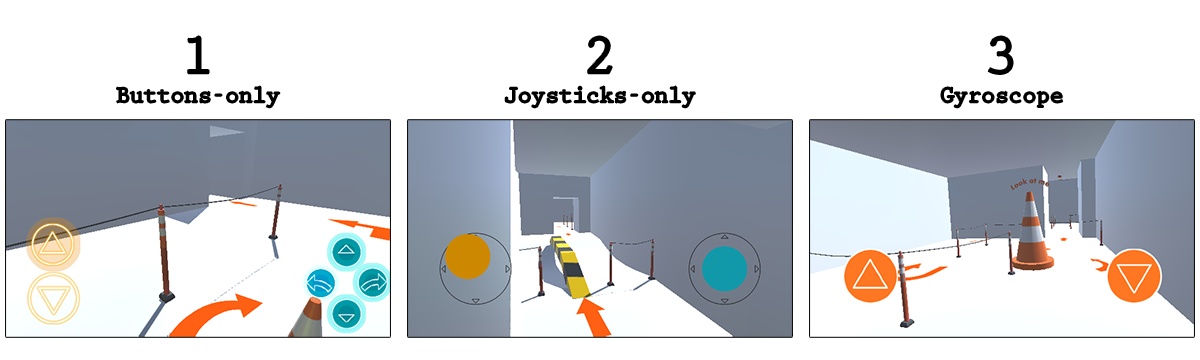
\includegraphics[width=.9\linewidth]{ControlSchemes.png}
  \captionof{figure}{Control Schemes}
\end{figure}

\subsection{Gyroscopic Controls}
Establishing the gyroscopic sensor creates a possibility to interact in an unusual but familiar way. It enables the prototype to be built around what is most familiar to the real life in movement; actually moving around in reality to navigate.
Controlling the camera with a built-in gyroscope in the tablet is familiar because it is a natural way for a person to look around. The forward and backward movements were implemented with on-screen buttons, as these were familiar to the target group through the usual human-computer interaction. Most of the controllers for movement are represented as this. E.g. arrows on the computer keyboard, music player, cell phone.
Such control scheme may have potential to engage the user in the task the most, if the user reaches the state of flow (\ref{FlowTheory}). \todo{fix labels}

\begin{figure}[H]
\centering
\begin{minipage}{.5\textwidth}
  \centering
  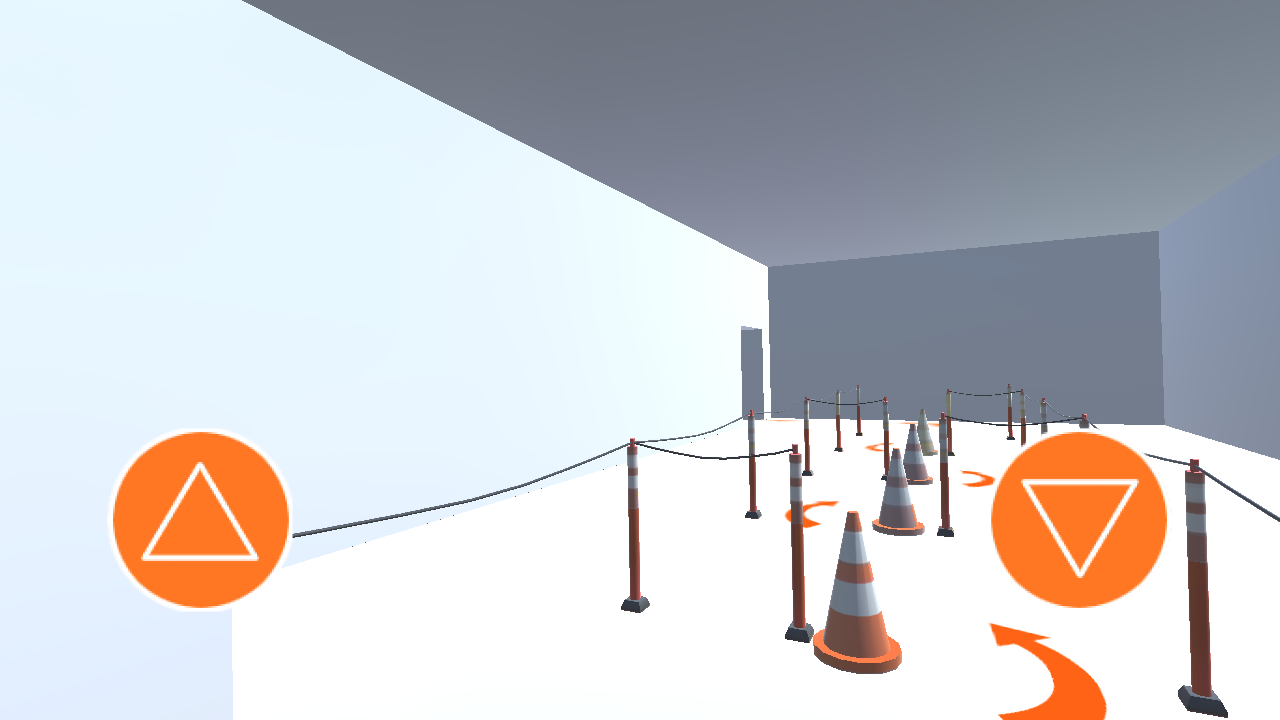
\includegraphics[width=.7\linewidth]{gyro1.png}
  \captionof{figure}{Initial sketch of gyroscope 1}
  \label{fig:test1}
\end{minipage}%
\begin{minipage}{.5\textwidth}
  \centering
  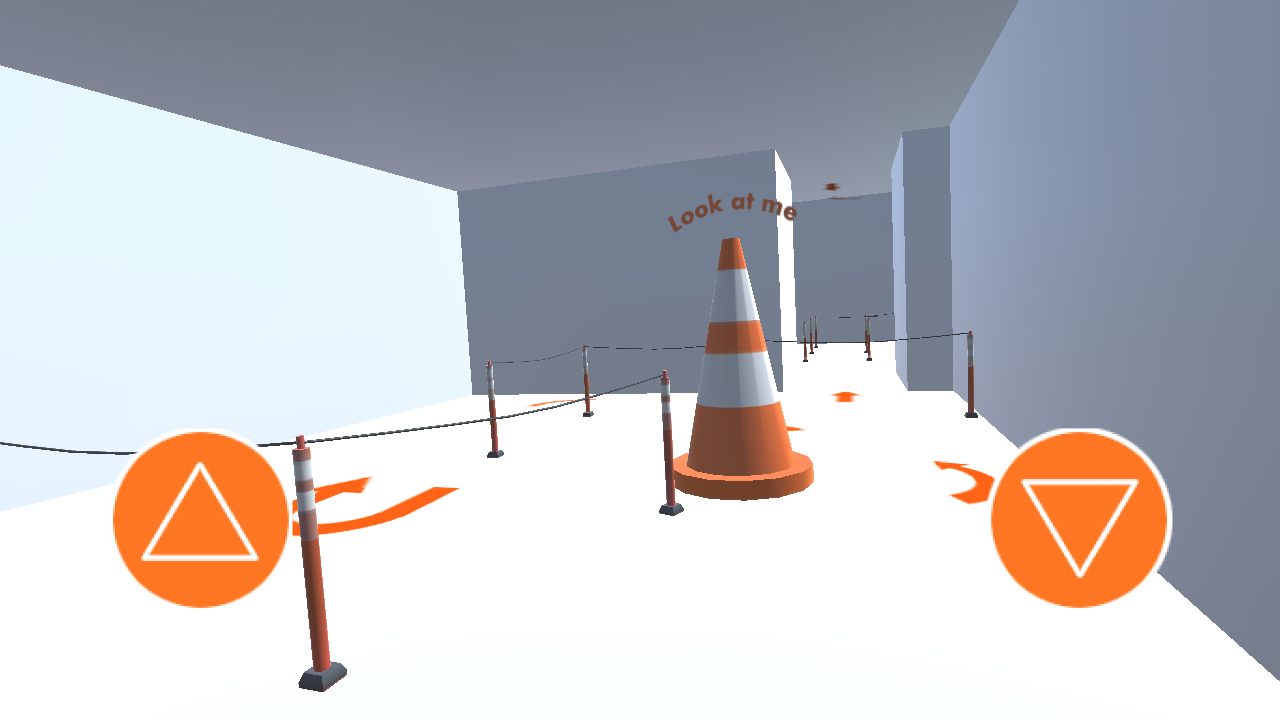
\includegraphics[width=.7\linewidth]{gyro2.png}
  \captionof{figure}{Initial sketch of gyroscope 2}
  \label{fig:test2}
\end{minipage}
\end{figure}


\subsection{Joystick}
In this prototype the user has to navigate using two joysticks - one for movement and one for the camera movement/rotation. This should be easy to learn for the users who have experienced using a joystick before. The target group is expected to have some knowledge of how a joystick is supposed to work, because of the popularity in arcade and electronic games where joysticks are placed on game console's remote controls, like Sony Playstation series or Microsoft Xbox. Even for users with no previous joystick controller experience, this should not be a problem. The control scheme is supposed to borrow the same concept as moving a computer mouse on the screen in the direction, both uses 2D directional movement.

\begin{figure}[H]
\centering
\begin{minipage}{.5\textwidth}
  \centering
  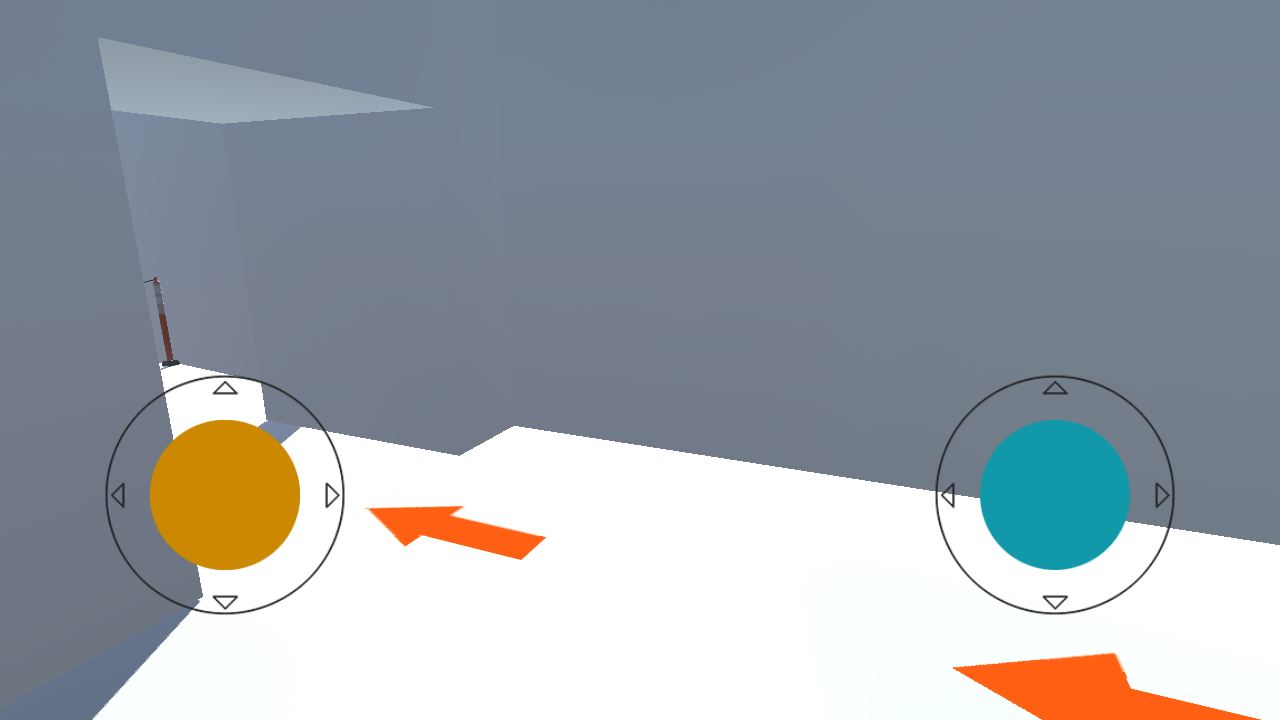
\includegraphics[width=.7\linewidth]{joystick1.png}
  \captionof{figure}{Initial sketch of joystick 1}
\end{minipage}%
\begin{minipage}{.5\textwidth}
  \centering
  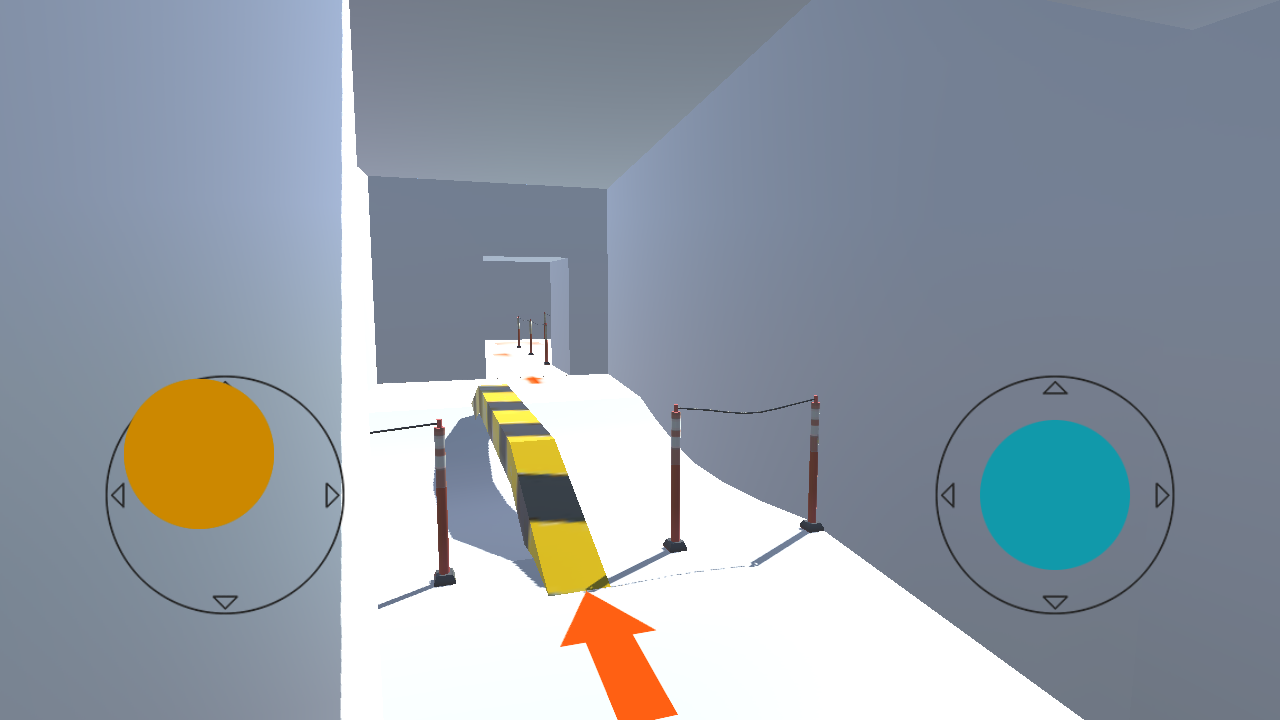
\includegraphics[width=.7\linewidth]{joystick2.png}
  \captionof{figure}{Initial sketch of joystick 2}
\end{minipage}
\end{figure}
\todo{what is the difference between these pics?}

\subsection{On-screen Buttons}
The control scheme that should be the most familiar for the users through daily use, only using buttons as the way to move both camera and the character. In this case, the camera would be moved only with arrow keys located on the screen and the same for moving around, arrows indicating movement back and forth. This should be familiar with anyone that has used buttons for navigation of any sorts in virtual environment. 

\begin{figure}[H]
\centering
\begin{minipage}{.5\textwidth}
  \centering
  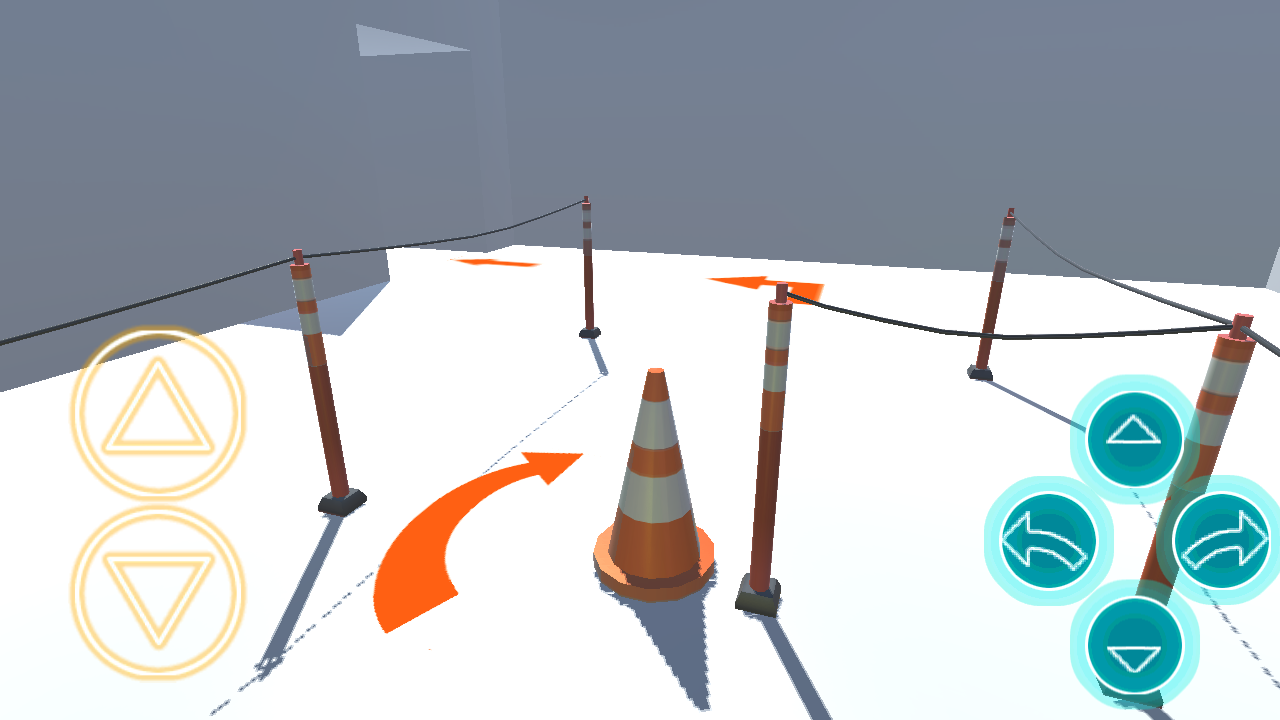
\includegraphics[width=.7\linewidth]{buttons1.png}
  \captionof{figure}{Initial sketch of buttons 1}
\end{minipage}%
\begin{minipage}{.5\textwidth}
  \centering
  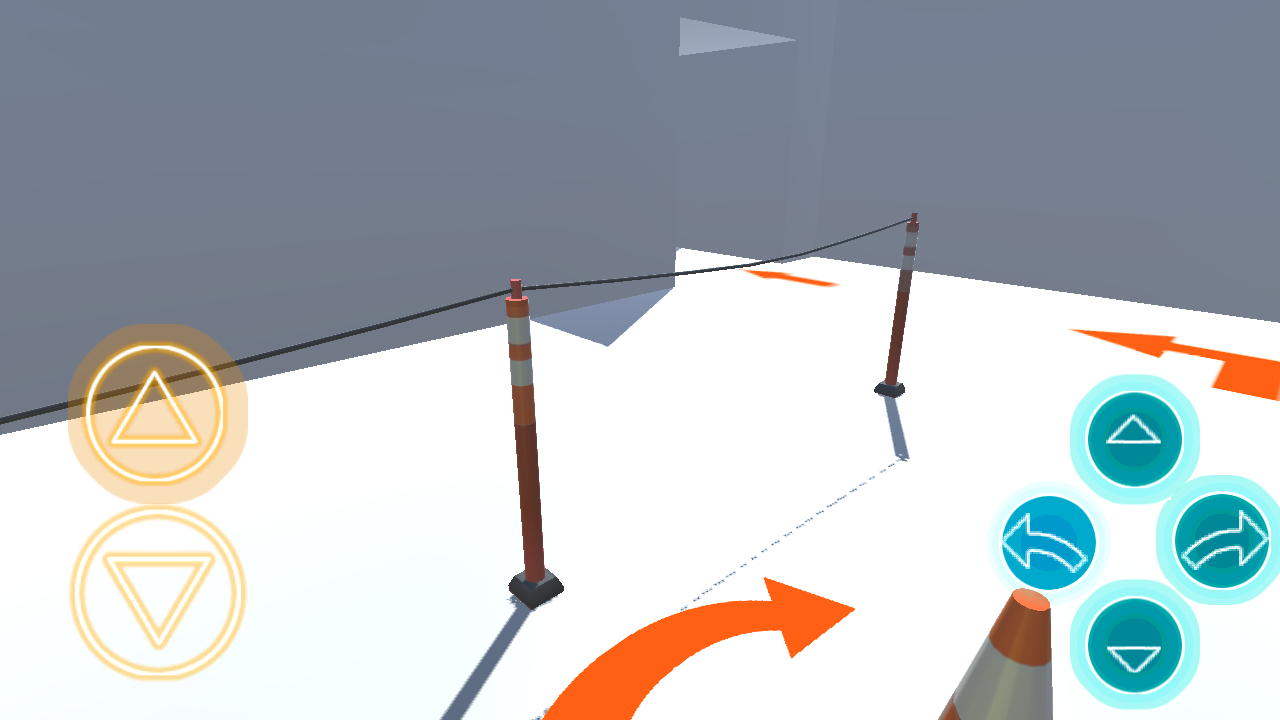
\includegraphics[width=.7\linewidth]{buttons2.png}
  \captionof{figure}{Initial sketch of buttons 2}
\end{minipage}
\end{figure}
\todo{no refs to pics - problem?}

\section{Isolation}
To further emphasize on the initial design requirements, the concept of isolation (\ref{GraphicalDesignIsolation} should be used when designing the controllers. This is done by making them stand out from the level content. This is supposed to help the user understand what parts of the application gives feedback upon interaction.

\section{Immediacy and Simplicity}
To communicate information faster and simpler, the designs should be represented by concepts that are already familiar to the user. This means, that to communicate information to the user, graphical elements should be represented as symbols that indicate either movement or rotation for buttons. Controls that represent an actual joystick, rather than
text. At the same time it emphasizes the concept of affordance \ref{UsabilityAffordance}, as the buttons represent mechanical buttons, as used in traditional types of controllers as well as with the joystick controls. This will further shape the intuition and familiarity for the application (\ref{UsabilityAffordance}.

\begin{figure}[H]
\centering
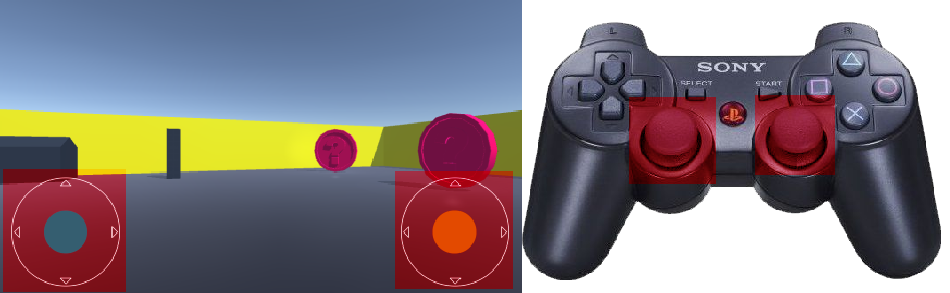
\includegraphics[scale=0.45]{JoystickComparison.png}
\caption{Comparison of initial design sketch of on-screen joystick and the Sony Playstation controller.}
\end{figure}

\section{Graphical element sizes and placement}
To further emphasize on the user experience, the button size should be set accordingly. To ensure that the users would not have difficulties by unintentionally tapping the wrong section of the controls (Section \ref{MobileUsability} mentions a case of Tetraplegia). Individual buttons have to be separated from each other and sized for easy accessibility to reduce the "Fat Finger" problem. To enable a bigger view of the environment horizontally, the application will be built to primarily be viewed when holding the device in a landscape mode. Since the device is supposed to be held sideways and by both hands, all of the interaction should be done on the sides of the screen for easy control access.
To show the difference between movement and rotation controls, they should be given different looks. Shapes of directional arrows for buttons as well as color indication for both buttons and joystick controls.

\begin{figure}[H]
\centering
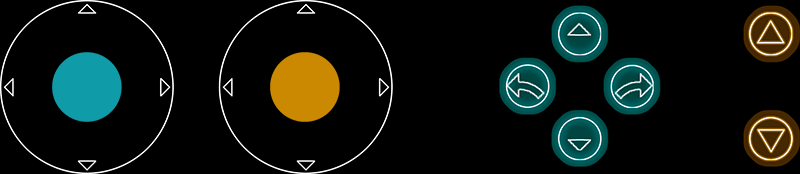
\includegraphics[scale=0.65]{ControllerColors.png}
\caption{Initial sketch. Colour differences to distinguish controllers that hold different functions.}
\end{figure}

\section{Design of 3D testing area}
To test different non-traditional control schemes a 3D test area was designed. It consists of a obstacles that test participants have to walk through as fast as possible \ref{TestLevels}.

\begin{figure}[H]
\centering
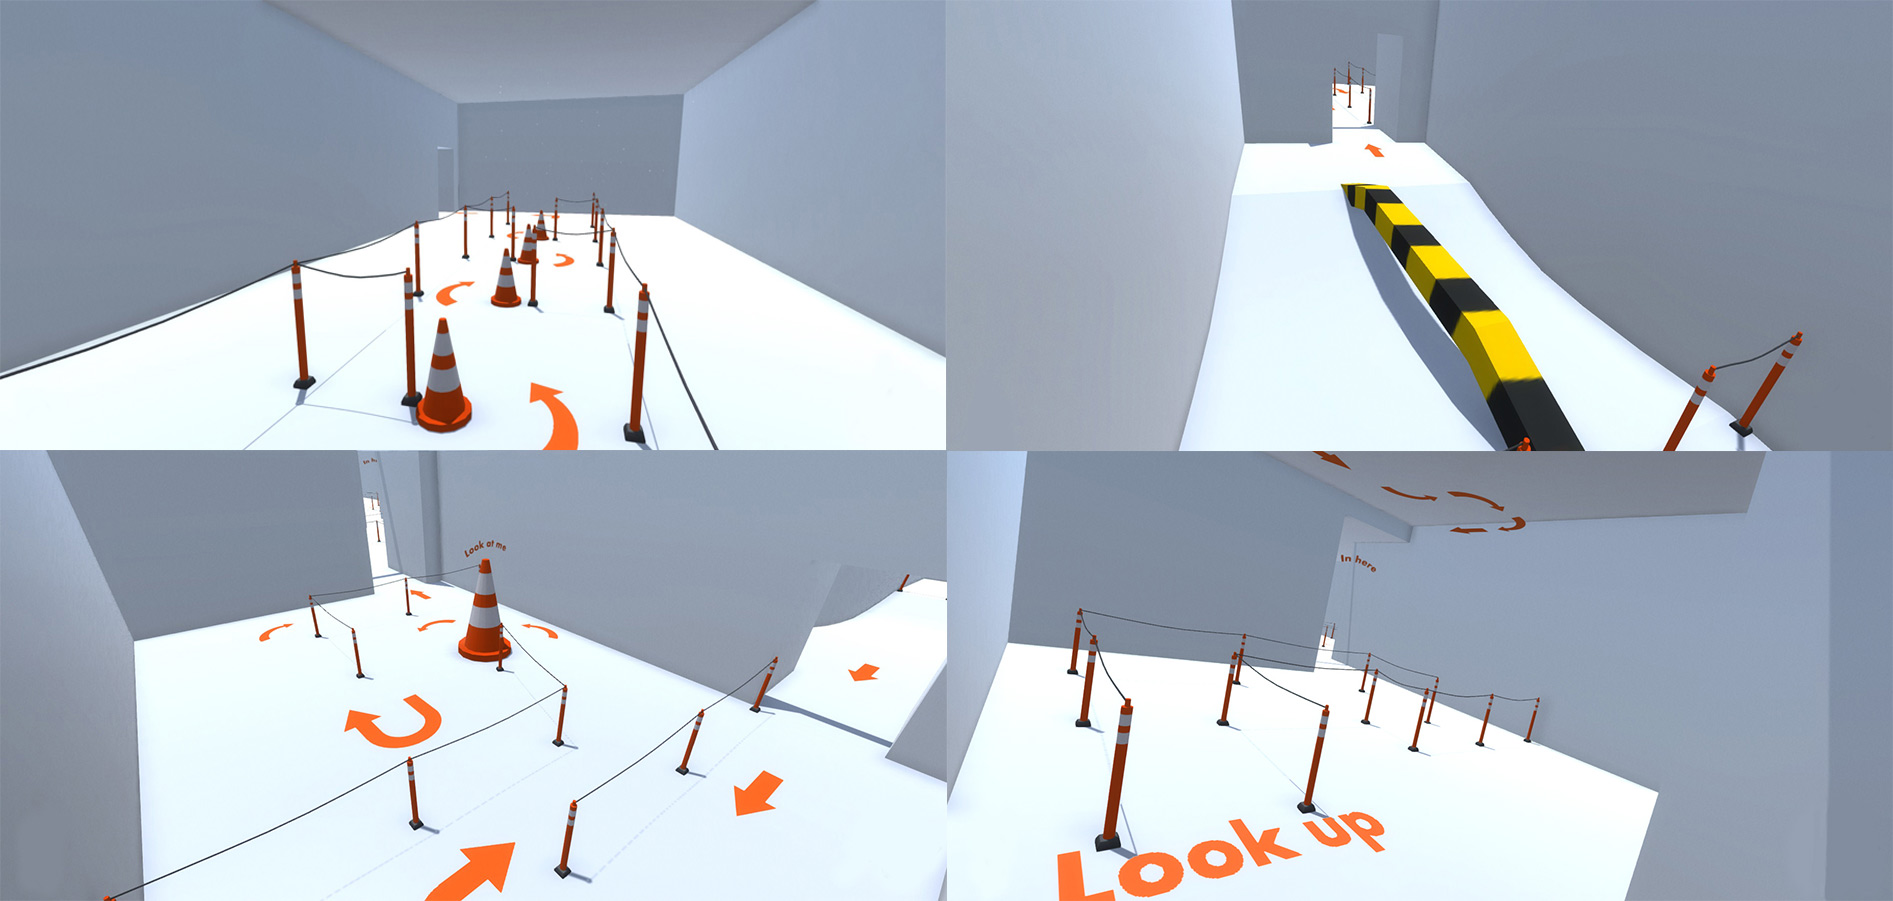
\includegraphics[scale=0.26]{3D_dev_6.jpg}
\caption{Pictures of the testing area}
\label{TestLevels}
\end{figure}

The focus of the testing area was only on navigation. So the tasks and obstacles was in focus and not the environment itself. All non-important bits of the area were coloured a white, neutral colour and important objects as navigational arrows, cones and poles and explanatory text notes, was coloured with a sharp contrasting colour e.g. red and orange. Navigational buttons and important objects in the level were kept in similar colours to help the user recognize and focus on the purpose. 
Analysing the state of the arts applications gave an understanding of what important aspects of navigation is.
\\
This helped to create \textbf{navigation testing goals.}
\subsubsection{Navigation testing goals}
\begin {enumerate}
\item First task is walking fluently around obstacles as doors, narrow paths. Second consideration was that the users need to look around placed objects. A small area with a big cone and text that said "look at me" was placed in the level with arrows in circular path around it. This represents how a user would walk around an object and inspect it by looking - focusing on one point while walking around \ref{TestLevel3}.

\begin{figure}[H]
\centering
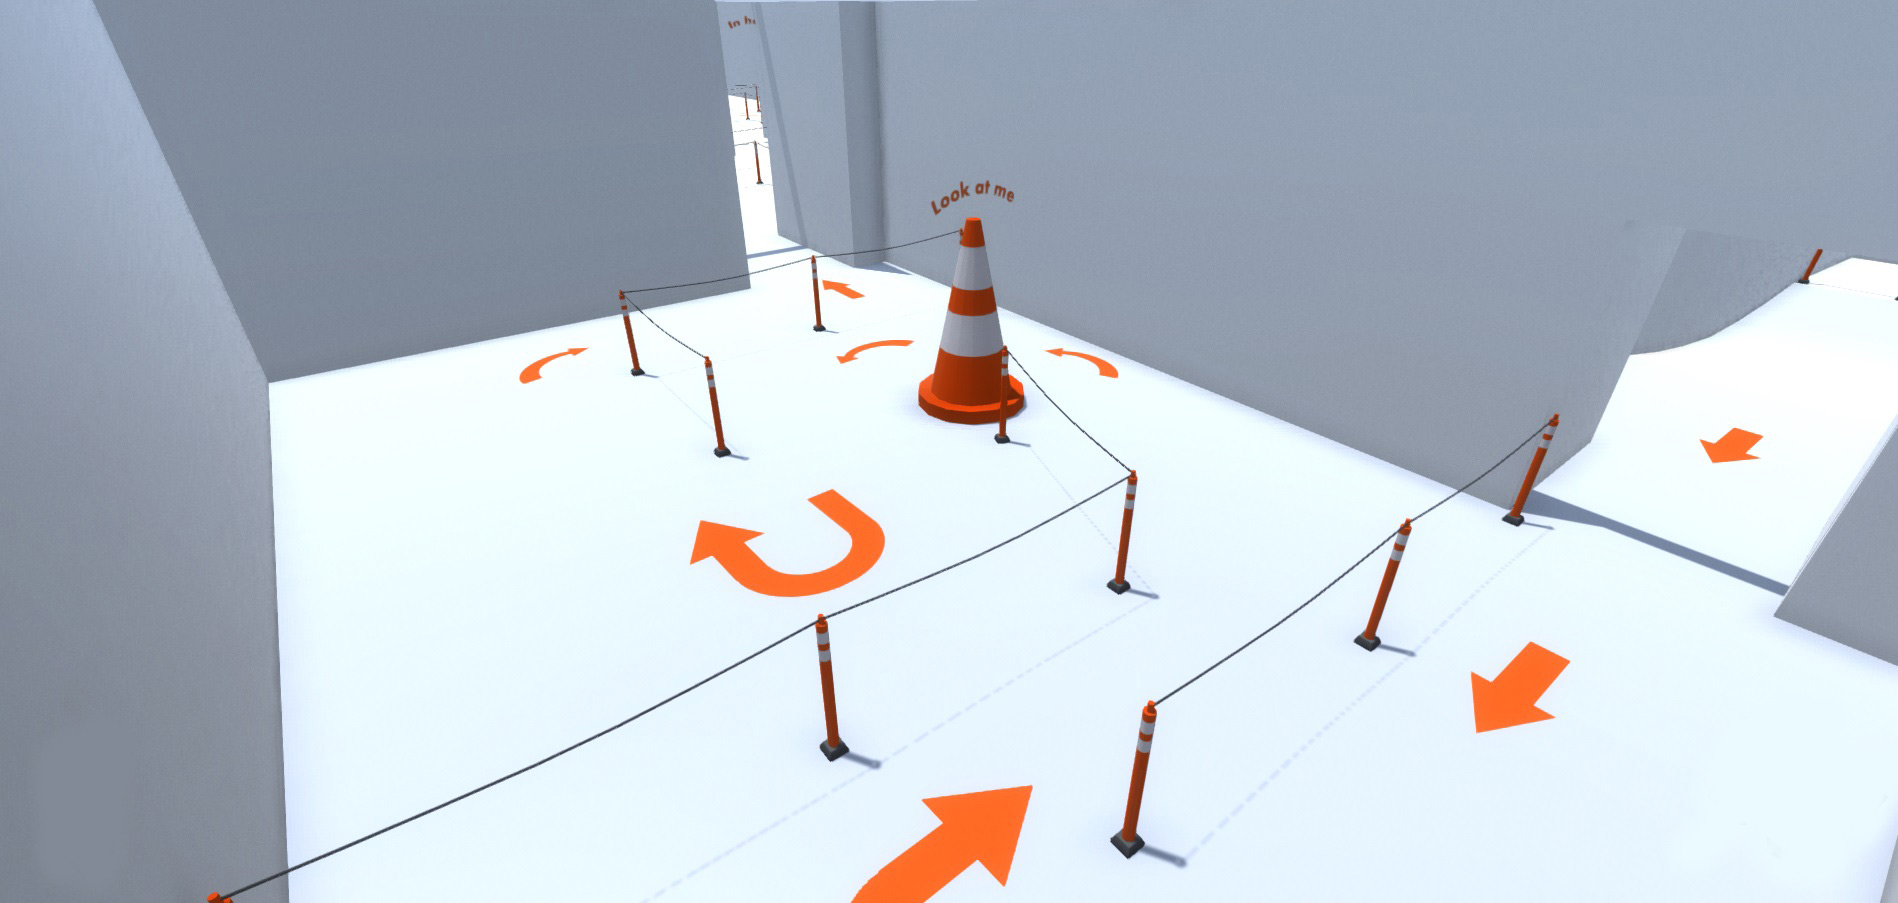
\includegraphics[scale=0.25]{3D_dev_3.jpg}
\caption{Third level of testing area. This level is to test how well the user walks around an object.}
\label{TestLevel3}
\end{figure}

\item The next two levels were developed to test how efficient it is to look up and down while walking in a given direction. It helps testing how well the user can walk while looking up or down at the same time \ref{TestLevel4}.

\begin{figure}[H]
\centering
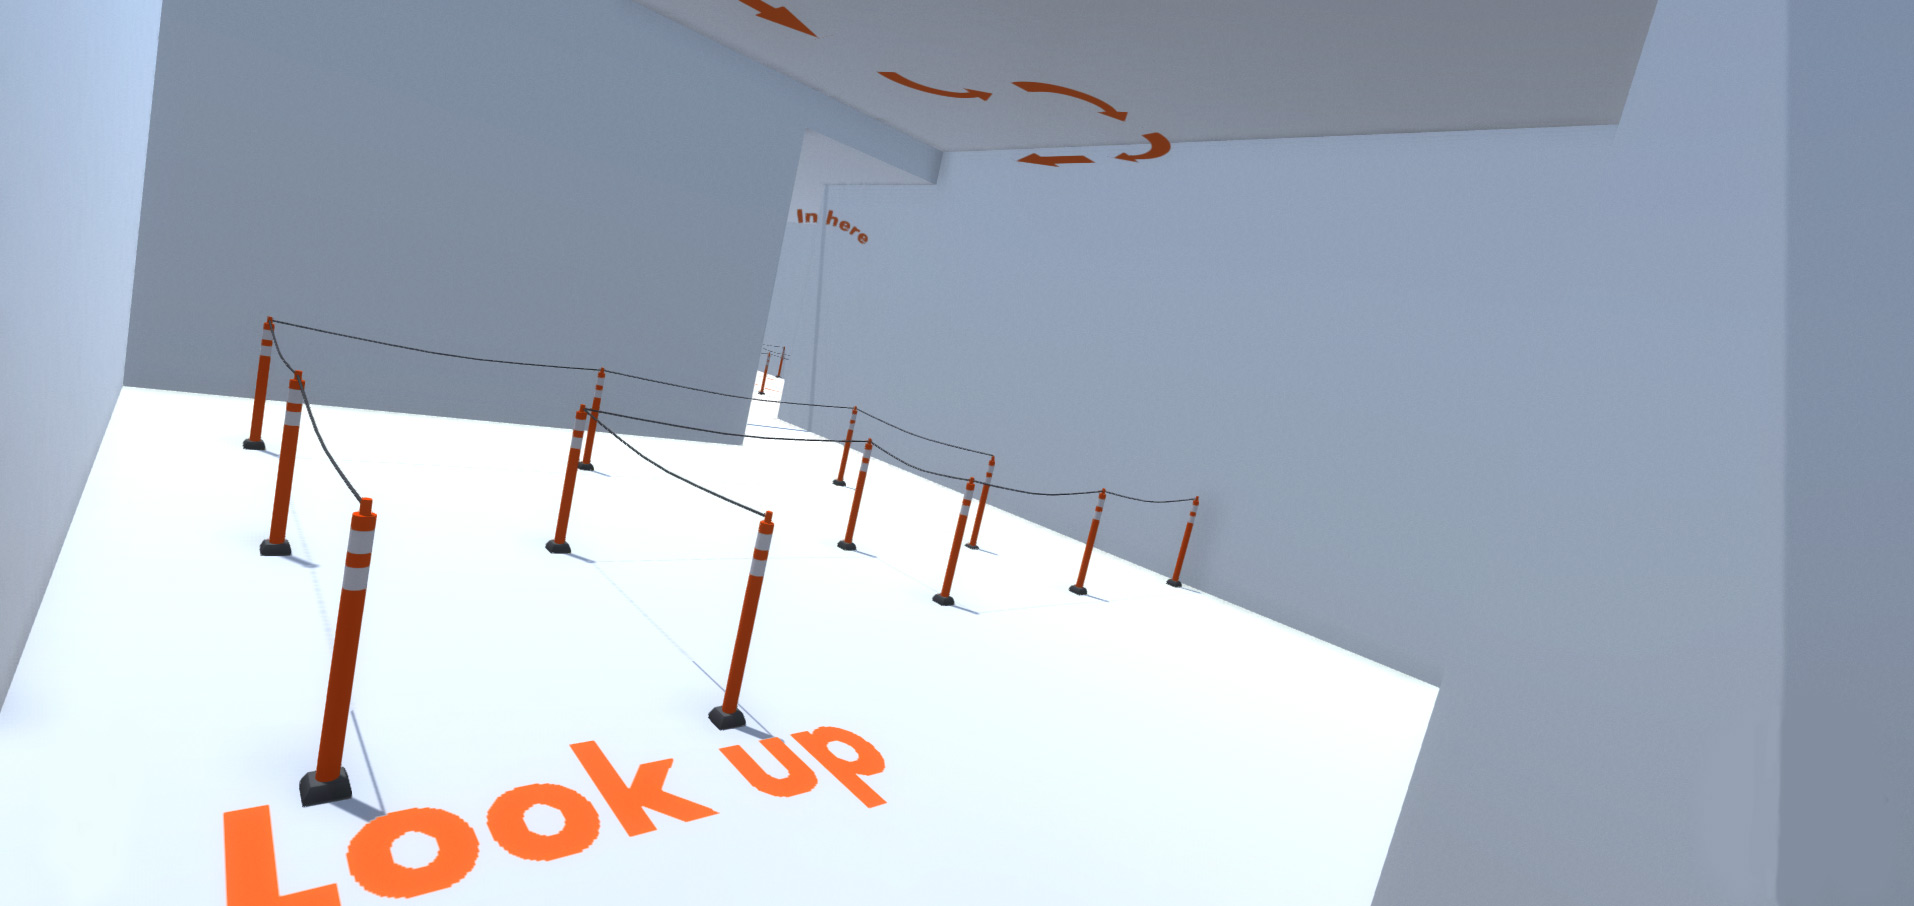
\includegraphics[scale=0.25]{3D_dev_4.jpg}
\caption{Test chamber to test how well user can walk and look up/down.}
\label{TestLevel4}
\end{figure}

\item The last test area was created to see how the user walks while looking to one side as the user would walk by \ref{TestLevel5}.

\begin{figure}[H]
\centering
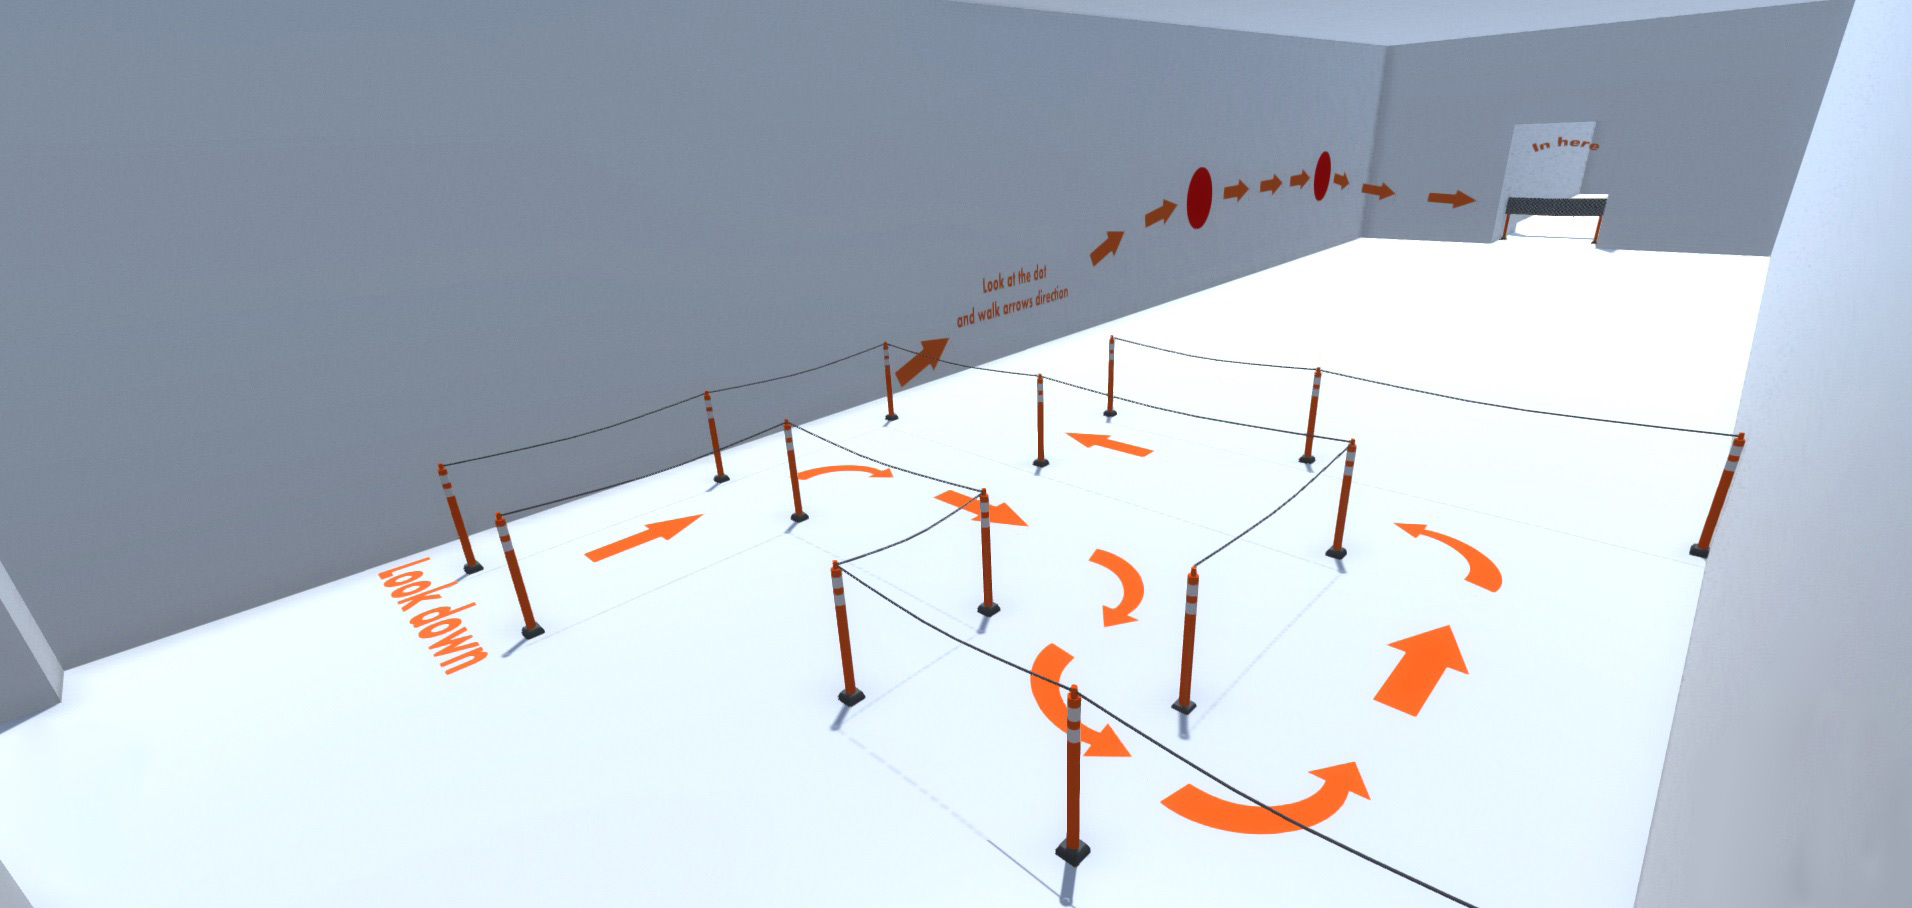
\includegraphics[scale=0.25]{3D_dev_5.jpg}
\caption{The last level of testing area. This level is to test how well the user can walk while looking down and sideways.}
\label{TestLevel5}
\end{figure}
\end{enumerate} 

\section{Design Conclusion}
Three distinct prototypes and a test level were designed for navigation in a 3D environment with all the initial design requirements in mind. With a goal to create a design that reduces the knowledge gap for the use the most. These initial prototypes will be implemented as three separate mobile applications for tablets and smartphones, with a gyroscopic sensor for the initial prototype testing. The designs will then be evaluated to help in the iterative design process.
In addition, these are not the only possible control schemes that the problem area covers, alternative design possibilities will be discussed in the discussion and redesign chapters in the report. 